\setcounter{chapter}{12}

\chapter{Generalized Linear Models}


{\small \textit{Chapter Preview}. This chapter describes a unifying
framework for the Part I linear model and the binary and count
models in Chapters 11 and 12. Generalized linear models, often known
by the acronym GLM, represent an important class of nonlinear
regression models that have found extensive use in actuarial
practice. This unifying framework not only encompasses many models
we have seen but also provides a platform for new ones, including
gamma regressions for fat-tailed data and ``Tweedie'' distributions
for two-part data.}

\section{Introduction}

There are many ways to extend, or generalize, the linear regression
model. This chapter introduces an extension that is so widely used
that it is known as \emph{the} ``generalized linear model,'' or as
the acronym GLM.

\index{symbols!$\eta$, systematic component}

Generalized linear models include linear, logistic and Poisson
regressions, all as special cases. One common feature of these
models is that in each case we can express the mean response as a
function of linear combinations of explanatory variables. In the GLM
context, it is customary to use $\mu_i = \mathrm{E}~y_i$ for the
mean response and call  $\eta_i = \mathbf{x}_i^{\mathbf{\prime}}
\boldsymbol \beta$ the \emph{systematic component} of the model. We
have seen that we can express the systematic component as:
\begin{itemize}
  \item $\mathbf{x}_i^{\mathbf{\prime}}
\boldsymbol \beta = \mu_i$, for (normal) linear regression,
  \item $\mathbf{x}_i^{\mathbf{\prime}}
\boldsymbol \beta = \exp(\mu_i)/(1+\exp(\mu_i)),$ for logistic
regression and
  \item $\mathbf{x}_i^{\mathbf{\prime}}
\boldsymbol \beta = \ln (\mu_i),$ for Poisson regression.
\end{itemize}
For GLMs, the systematic component is related to the mean through
the expression
\begin{equation}\label{E13: Link}
\eta _i = \mathbf{x}_i^{\mathbf{\prime}} \boldsymbol \beta =
\mathrm{g}\left( \mu _i\right).
\end{equation}
Here, g(.) is known and called the \emph{link} function. The inverse
of the link function, $\mu _i = \mathrm{g}^{-1}(
\mathbf{x}_i^{\mathbf{\prime}} \boldsymbol \beta)$, is the mean
function.\index{link function}

The second common feature involves the distribution of the dependent
variables. In Section \ref{S13:GLMModel}, we will introduce the
\emph{linear exponential family of distributions}, an extension of
the exponential distribution. This family includes the normal,
Bernoulli and Poisson distributions as special cases.

The third common feature of GLM models is the robustness of
inference to the choice of distributions. Although linear regression
is motivated by normal distribution theory, we have seen that
responses need not be normally distributed for statistical inference
procedures to be effective. The Section 3.2 sampling assumptions
focus on:
\begin{itemize}
  \item the form of the mean function (assumption F1),
  \item non-stochastic or exogenous explanatory variables (F2),
  \item constant variance (F3) and
  \item independence among observations (F4).
\end{itemize}
GLM models maintain assumptions F2 and F4 and generalize F1 through
the link function. The choice of different distributions allows us
to relax F3 by specifying the variance to be a function of the mean,
written as $\mathrm{Var~}y_i = \phi v(\mu_i)$. Table
\ref{T13:VarianceFunctions} shows how the variance depends on the
mean for different distributions. As we will see when considering
estimation (Section \ref{S13:Estimation}), it is the choice of the
variance function that drives the most important inference
properties, not the choice of the distribution.

\marginparjed{The choice of the variance function drives many
inference properties, not the choice of the distribution.}

\index{symbols!$v(\cdot)$, variance function}

\begin{table}[h]
\caption{\label{T13:VarianceFunctions} Variance Functions for
Selected Distributions} \scalefont{0.9}
\begin{tabular}{lc}
\hline
Distribution & Variance Function $v(\mu)$ \\
\hline
Normal & 1 \\
Bernoulli & $\mu ( 1- \mu ) $ \\
Poisson & $\mu $ \\
Gamma & $\mu ^2 $ \\
Inverse Gaussian & $\mu ^3 $ \\
\hline
\end{tabular}
\scalefont{1.1111}
\end{table}


By considering regression in the GLM context, we will be able to
handle dependent variables that are approximately normally
distributed, binary or representing counts, all within one
framework. This will aid our understanding of regression by allowing
us to see the ``big picture'' and not be so concerned with the
details. Further, the generality of GLMs will allow us to introduce
new applications, such as gamma regressions that are useful for
fat-tailed distributions and the so-called ``Tweedie'' distributions
for two-part data. Two-part data is a topic taken up in Chapter 16,
where there is a mass at zero and a continuous component. For
insurance claims data, the zero represents no claim and the
continuous component represents the amount of a claim.

This chapter describes estimation procedures for calibrating GLM
models, significance tests and goodness of fit statistics for
documenting the usefulness of the model, and residuals for assessing
the robustness of the model fit. We will see that the our earlier
work done on linear, binary and count regression models provides the
foundations for the tools needed for the GLM model. Indeed, many are
slight variations of tools and concepts developed earlier in this
text and we will be able to build on these foundations.


\section{GLM Model}\label{S13:GLMModel}\index{regression model!generalized linear model, $GLM$}

To specify a GLM, the analyst chooses an underlying response
distribution, the topic of Section \ref{S13:LinExpFam}, and a
function that links the mean response to the covariates, the topic
of Section \ref{S13:LinkFunction}.

\subsection{Linear Exponential Family of
Distributions}\label{S13:LinExpFam}\index{distributions! linear
exponential family}

\bigskip
\begin{center}
\boxedjed

\textit{Definition.} The distribution of the \emph{linear
exponential family} is
\begin{equation}\label{E13:LinearExpFam}
\mathrm{f}( y; \theta ,\phi ) =\exp \left( \frac{y\theta -b(\theta )}{\phi }%
+S\left( y,\phi \right) \right).
\end{equation}
Here, $y$ is a dependent variable and $\theta $ is the parameter of
interest. The quantity $\phi $ is a scale parameter. The term $b(\theta )$ depends only
on the parameter $\theta$, not the dependent variable. The statistic $S\left( y,\phi \right) $ is a
function of the dependent variable and the scale parameter, not the
parameter $\theta $.

\end{boxedminipage}
\end{center}
\bigskip

The dependent variable $y$ may be discrete, continuous or a mixture.
Thus, $\mathrm{f} \left( .\right) $ may be interpreted to be a
density or mass function, depending on the application. Table
\ref{T13:SelDistns} provides several examples, including the normal,
binomial and Poisson distributions. To illustrate, consider a
normal distribution with a probability density function of the form%
\begin{eqnarray*}
\mathrm{f}( y; \mu ,\sigma ^{2})  &=&\frac{1}{\sigma \sqrt{2\pi
}}\exp \left( -
\frac{(y-\mu )^{2}}{2\sigma ^{2}}\right)  \\
&=&\exp \left( \frac{(y\mu -\mu ^{2}/2)}{\sigma ^{2}}-\frac{y^{2}}{2\sigma
^{2}}-\frac{1}{2}\ln \left( 2\pi \sigma ^{2}\right) \right) .
\end{eqnarray*}
With the choices $\theta =\mu $, $\phi =\sigma ^{2}$, $b(\theta
)=\theta ^{2}/2$ and $S\left( y,\phi \right) =-y^{2}/(2\phi )-\ln
\left( 2\pi \phi \right) /2$, we see that the normal probability
density function can be expressed as in equation
(\ref{E13:LinearExpFam}).

For the distribution in equation (\ref{E13:LinearExpFam}), some
straightforward calculations show that
\begin{itemize}
\item $\mathrm{E~}y=b^{\prime }(\theta )$ and
\item $\mathrm{Var~}y=\phi b^{\prime \prime }(\theta )$.
\end{itemize}
For reference, these calculations appear in Section
\ref{S13:Moments}. To illustrate, in the context of the normal
distribution example above, it is easy to check that
$\mathrm{E~}y=b^{\prime }(\theta )=\theta =\mu $ and $\mathrm{Var~}
y = \sigma ^{2}b^{\prime \prime }(\theta )=\sigma ^{2}$, as
anticipated.

In regression modeling situations, the distribution of $y_i$ varies
by observation through the subscript ``$i$''.  It is customary to let the
distribution family remain constant yet allow
the parameters to vary by observation through the notation
$\theta_i$ and $\phi_i$. For our applications, the variation of the
scale parameter is due to known weight factors. Specifically, when
the scale parameter varies by observation, it is according to $\phi
_i=\phi /w_i$, that is, a constant divided by a known weight $w_i$.
With the relation $\mathrm{Var~}y_i=\phi_i b^{\prime \prime
}(\theta_i)=\phi b^{\prime \prime }(\theta_i)/w_i$, we have that a
larger weight implies a smaller variance, other things being equal.

\subsection{Link Functions}\label{S13:LinkFunction}

In regression situations, we wish to understand the impact of
$\eta_i = \mathbf{x}_i^{\mathbf{\prime}} \boldsymbol \beta$, the
systematic component. As we saw in the prior subsection, we can
express the mean of $y_i$ as $\mathrm{E~}y_i=\mu _i=b^{\prime
}(\theta_i)$. Equation (\ref{E13: Link}) serves to ``link'' the
systematic component to $\mu_i$ and thus to the parameter
$\theta_i$. It is possible to use the identity function for g(.) so
that $\mu _i=b^{\prime }(\theta_i)$. Indeed, this is the usual case
in linear regression. However, linear combinations of explanatory
variables, $\mathbf{x}_i^{\mathbf{\prime }}\boldsymbol \beta$, may
vary between negative and positive infinity whereas means are often
restricted to smaller range. For example, Poisson means vary between
zero and infinity. The link function serves to map the domain of the
mean function onto the whole real line.

\linejed

\textbf{Special Case: Links for the Bernoulli distribution}.
Bernoulli means are probabilities and thus vary between zero and
one. For this case, it is useful to choose a link function that maps
the unit interval (0,1) onto the whole real line. The following are
three important examples of link functions for the Bernoulli
distribution:

\begin{itemize}
\item Logit: $g(\mu )=\mathrm{logit}(\mu )=\ln (\mu /(1-\mu ))$ .

\item Probit: $g(\mu )=\Phi ^{-1}(\mu )$, where $\Phi ^{-1}$ is the inverse
of the standard normal distribution function.

\item Complementary log-log: $g(\mu )=\ln \left( -\ln (1-\mu )\right) $.
\end{itemize}

\linejed

This illustration demonstrates that there may be several link
functions that are suitable for a particular distribution. To help
with the selection, an intuitively appealing case occurs when the
systematic component equals the
parameter of interest ($\eta =\theta $). To see this, first recall that $%
\eta =g(\mu )$ and $\mu =b^{\prime }(\theta )$, dropping the ``$i$''
subscripts for the moment. Then, it is easy to see that if
$g^{-1}=b^{\prime }$, then $\eta =g(b^{\prime }(\theta ))=\theta $.
The choice of $g$ that is the inverse of $b^{\prime }(\theta )$ is
called the \emph{canonical link}.\index{link function!canonical}

\marginparjed{The choice of $g$ that is the inverse of $b^{\prime
}(\theta )$ is called the canonical link. With this choice, the
systematic component equals the parameter of interest.}

Table \ref{T13:MeanLinks} shows the mean function and corresponding
canonical link for several important distributions.

\begin{table}[h]
\caption{\label{T13:MeanLinks} Mean Functions and Canonical Links
for Selected Distributions} \scalefont{0.9}
\begin{tabular}{lcc}
\hline Distribution & Mean function $b^{\prime }(\theta )$  &
Canonical link $g(\mu )$  \\ \hline
Normal & $\theta $ & $ \mu $ \\
Bernoulli & $ e^{\theta}/(1+e^{\theta} )$
& $\mathrm{logit}(\mu )$ \\
Poisson & $ e^{\theta }$ & $\ln  \mu $ \\
Gamma & $-1/\theta$ & $-1/\mu $ \\
Inverse Gaussian & $(-2 \theta )^{-1/2} $ & $-1 /(2 \mu^2) $ \\
\hline
\end{tabular}
\scalefont{1.1111}
\end{table}

\noindent Links relate the mean to the systematic component and to
the regression parameters. Because the regression parameters are
unknown, it is common to specify the links only up to scale. For
example, it is common to specify the inverse gaussian canonical link
as $1 /\mu^2$ (instead of $-1 /(2 \mu^2) $). If necessary, one can
always recover the scale when estimating the unknown regression
coefficients.

\empexjed{AutoCollision}\index{datasets!automobile UK collision}

\linejed\index{actuarial \& financial terms and concepts!ratemaking}

\textbf{Example: Ratemaking Classification.} The process of grouping
risks with similar characteristics is known as \emph{risk
classification}. \emph{Ratemaking} is the art of setting premiums,
or rates, based on loss experience and exposures of risk classes.
For example, Mildenhall (1999) considered 8,942 collision losses
from private passenger United Kingdom (UK) automobile insurance
policies. The data were derived from Nelder and McCullagh (1989,
Section 8.4.1) but originated from Baxter et al. (1980). A typical
personal auto rating plan is based on driver and vehicle
characteristics. Driver characteristics may include the driver's
age, gender, marital status, history (accidents and violations) and
good student discount. Vehicle characteristics may include vehicle
model type and year, purpose (business/school or pleasure), garage
territory and so forth. We can represent the systematic component as
\begin{equation*}
\eta_{ij} = \beta_0 + \alpha_i + \tau_j,
\end{equation*}
where $\alpha_i$ represents the effect of the $i$th category of
driver classification and $\tau_j$ the effect of the $j$th vehicle
type. Table \ref{T13:PrivateCollision} displays the Mildenhall data
for eight driver types (age groups) and four vehicle classes
(vehicle use). The average severity is in pounds sterling adjusted
for inflation.

\index{actuarial \& financial terms and concepts!ratemaking!additive
plan} \index{actuarial \& financial terms and
concepts!ratemaking!multiplicative plan}

In GLM terminology, an \emph{additive rating plan} is based on the
identity link function whereas a \emph{multiplicative plan} is based
on a logarithmic link function. Specifically, if we use $ \eta_{ij}
= \ln ( \mu _{ij}) $, then we can write the mean as
\begin{equation}\label{E13:MultiplicativePrems}
\mu _{ij} = \exp(\beta_0 + \alpha_i + \tau_j) = B \times A_i \times
T_j,
\end{equation}
where $B=\exp(\beta_0)$ is a scaling constant, $A_i=\exp(\alpha_i)$
represents driver effects and  $T_j=\exp(\tau_j)$ represents vehicle
effects.


\begin{table}[h]
\scalefont{0.9} \caption{\label{T13:PrivateCollision} Private
Passenger Automobile UK Collision Data}
\begin{tabular}{lcrr|llcrr}
 \hline
       Age &   Vehicle  &    Average &      Claim &~~~ &       Age &   Vehicle  &    Average &      Claim \\
     Group &        Use &   Severity &      Count & &     Group &        Use &   Severity &      Count \\
     \hline
     17-20 &   Pleasure &     250.48 &         21 &  &     35-39 &   Pleasure &     153.62 &        151 \\
     17-20 & DriveShort &     274.78 &         40 & &      35-39 & DriveShort &     201.67 &        479 \\
     17-20 &  DriveLong &     244.52 &         23 & &      35-39 &  DriveLong &     238.21 &        381 \\
     17-20 &   Business &     797.80 &          5 & &      35-39 &   Business &     256.21 &        166 \\
 \hline
     21-24 &   Pleasure &     213.71 &         63 & &      40-49 &   Pleasure &     208.59 &        245 \\
     21-24 & DriveShort &     298.60 &        171 & &      40-49 & DriveShort &     202.80 &        970 \\
     21-24 &  DriveLong &     298.13 &         92 & &      40-49 &  DriveLong &     236.06 &        719 \\
     21-24 &   Business &     362.23 &         44 & &     40-49 &   Business &     352.49 &        304 \\
 \hline
     25-29 &   Pleasure &     250.57 &        140 & &      50-59 &   Pleasure &     207.57 &        266 \\
     25-29 & DriveShort &     248.56 &        343 & &      50-59 & DriveShort &     202.67 &        859 \\
     25-29 &  DriveLong &     297.90 &        318 & &      50-59 &  DriveLong &     253.63 &        504 \\
     25-29 &   Business &     342.31 &        129 &  &     50-59 &   Business &     340.56 &        162 \\
 \hline
     30-34 &   Pleasure &     229.09 &        123 & &        60+ &   Pleasure &     192.00 &        260 \\
     30-34 & DriveShort &     228.48 &        448 & &        60+ & DriveShort &     196.33 &        578 \\
     30-34 &  DriveLong &     293.87 &        361 & &        60+ &  DriveLong &     259.79 &        312 \\
     30-34 &   Business &     367.46 &        169 & &        60+ &   Business &     342.58 &         96 \\
 \hline
 \multicolumn{9}{l}{\textit{Source}: Mildenhall (1999). ``DriveShort'' means drive to work but less than 10
 miles.} \\
  \multicolumn{9}{l}{``DriveLong'' means drive to work but more than 10 miles.}
\end{tabular}
\linetjed \scalefont{1.1111}
\end{table}



\section{Estimation}\label{S13:Estimation}

This section presents maximum likelihood, the customary form of
estimation. To provide intuition, we focus on the simpler case of
canonical links. Results for more general links appear in Section
\ref{S13:MLEGeneralLinks}.

\subsection{Maximum Likelihood Estimation for Canonical
Links}\label{S13:MLECanonLinks}

\index{likelihood inference!log-likelihood}\index{likelihood
inference!score function}\index{likelihood inference!maximum
likelihood estimator}

From equation (\ref{E13:LinearExpFam}) and the independence among
observations, the log-likelihood is
\begin{equation}\label{E13:LogLike}
\ln \mathrm{f}( \mathbf{y}) =\sum_{i=1}^n
 \left\{
\frac{y_i\theta_i-b(\theta_i)}{\phi _i}+S( y_i,\phi _i ) \right\} .
\end{equation}
Recall that for canonical links, we have equality between the
distribution's parameter and the systematic component, so that
$\theta_i=\eta _i=\mathbf{x}_i^{\mathbf{\prime }}\boldsymbol \beta$.
Thus, with $\phi _i=\phi /w_i$, the log-likelihood is
\begin{equation}\label{E13:LogLikeCanonLink}
L (\boldsymbol \beta, \phi ) = \ln \mathrm{f}( \mathbf{y})
=\sum_{i=1}^n \left\{ \frac{y_i\mathbf{x}
_i^{\mathbf{\prime }}\boldsymbol \beta-b(\mathbf{x}_i^{\mathbf{\prime }}%
\boldsymbol \beta)}{\phi / w_i}+S( y_i,\phi / w_i) \right\} .
\end{equation}
Taking the partial derivative with respect to $\boldsymbol \beta$
yields the score function
\begin{equation}\label{E13:GLMScore}
\frac{\partial }{\partial \boldsymbol \beta} L( \boldsymbol \beta,
\phi ) = \frac{1}{\phi} \sum_{i=1}^n \left( y_i-b^{\prime
}(\mathbf{x} _i^{\mathbf{\prime }}\boldsymbol \beta) \right) w_i
\mathbf{x}_i .
\end{equation}
Because $\mu _i=b^{\prime }(\theta_i)=b^{\prime }(\mathbf{x}_i^{%
\mathbf{\prime }}\boldsymbol \beta)$, we can solve for the maximum
likelihood estimators of $\boldsymbol \beta$, $\mathbf{b}_{MLE} $,
through the ``normal equations''
\begin{equation}\label{E13:GLMNormalEqn}
\mathbf{0}=\sum_{i=1}^n w_i \left( y_i-\mu _i\right) \mathbf{x}_i.
\end{equation}\index{normal equations} There are $k+1$ equations and $k+1$
unknowns in the equation (\ref{E13:GLMNormalEqn}). Typically, the
solution is unique and we use the notation $\mathbf{b}_{MLE}$ to
denote the solution. One reason for the widespread use of GLM
methods is that the maximum likelihood estimators can be computed
quickly through a technique known as \emph{iterated reweighted least
squares}, described in Section \ref{S13:IterRWLS}.\index{least
squares!iterated reweighted}

Note that, like ordinary linear regression normal equations, we do
not need to consider estimation of the variance scale parameter
$\phi $ at this stage. That is, we can first compute
$\mathbf{b}_{MLE}$ and, when necessary, estimate $\phi $. ($\phi$ is
known for certain distributions such as the binomial and Poisson and
so does not require estimation.)

As described in Section 11.9%\ref{S11:LikelihoodInference}
, maximum likelihood estimators are consistent and have large sample
normal distributions under broad conditions. Maximum likelihood
inference provides a mechanism for calculating this distribution.
From equations (\ref{E13:GLMScore}) and the likelihood technical
supplement (Section 11.9, equation 11.14), the corresponding
information matrix is
\begin{equation} \label{E13:StdErrors}
\mathbf{I} \left( \mathbf{b}_{MLE} \right) =
\frac{1}{\phi}\sum_{i=1}^n w_i ~b^{\prime \prime }(\mathbf{x}_i
^{\mathbf{\prime }} \mathbf{b}_{MLE} ) ~ \mathbf{x}_i
\mathbf{x}_i^{\mathbf{\prime }} .
\end{equation}
The inverse of the information matrix is the large sample
variance-covariance matrix of $\mathbf{b}_{MLE}$. Specifically, the
square root of the $(j+1)$st diagonal element of the inverse of this
matrix yields the standard error for $b_{j,MLE}$, which we denote as
$se(b_{j,MLE})$. Extensions to general links are
similar.\index{likelihood inference!information matrix}

Inference for $\mathbf{b}_{MLE}$ is robust to the choice of
distributions in the following sense. The solution of the maximum
likelihood estimators in equation (\ref{E13:GLMNormalEqn}) only
depends on the mean function; it can be shown that consistency of
the estimators depends only on proper choice of this function.
Further, the large sample behavior of $\mathbf{b}_{MLE}$ essentially
only requires that the mean and variance functions be correctly
specified, not the choice of the distribution. (A few additional
regularity conditions are required but these are mild technical
requirements.) For example, suppose an analyst chooses a Poisson
distribution with a logarithmic link. If the log link is
appropriate, then only the equality between the mean and the
variance is needed, see Table \ref{T13:VarianceFunctions}. Unlike
the usual domain of the Poisson distribution, the dependent
variables could be non-integers or even be negative. Large sample
inference for $\mathbf{b}_{MLE}$ only requires that we choose the
mean and variance functions correctly.

\linejed

\textbf{Example: Ratemaking Classification - Continued.} Using the
data in Table \ref{T13:PrivateCollision}, a log-link function with
gamma distribution was fit using claim counts as weights ($w_i$).
Table \ref{T13:PrivateCollisionRates} shows estimates of the
expected severity using equation (\ref{E13:MultiplicativePrems}).
The averages suggest that young drivers (ages 17-20 and 21-24) have
the highest claims. For vehicle use, those driving for pleasure had
the lowest and those driving for business had the highest claims.

\begin{table}[h]
\scalefont{0.9} \caption{\label{T13:PrivateCollisionRates} Estimated
Expected Severity for a Multiplicative Rating Plan}
\begin{tabular}{l|rrrr|r}
\hline
 Age Group   & DriverShort &  DriveLong &   Pleasure &   Business &    Average \\
\hline
     17-20 &     322.17 &     265.56 &     254.90 &     419.07 &     315.42 \\
     21-24 &     320.66 &     264.31 &     253.70 &     417.10 &     313.94 \\
     25-29 &     297.26 &     245.02 &     235.19 &     386.66 &     291.03 \\
     30-34 &     284.85 &     234.80 &     225.37 &     370.53 &     278.89 \\
     35-39 &     229.37 &     189.06 &     181.47 &     298.35 &     224.56 \\
     40-49 &     248.15 &     204.54 &     196.33 &     322.78 &     242.95 \\
     50-59 &     251.95 &     207.67 &     199.34 &     327.72 &     246.67 \\
       60+ &     246.47 &     203.16 &     195.00 &     320.60 &     241.31 \\
\hline
   Average &     275.11 &     226.77 &     217.66 &     357.85 &     269.35 \\
\hline
\end{tabular}\scalefont{1.1111}

\linetjed
\end{table}


\subsection{Overdispersion}\index{dispersion!overdispersion}

For some members of the linear exponential family, such as the
Bernoulli and the Poisson distributions, the variance is determined
by the mean. In contrast, the normal distribution has a separate
scale parameter. When fitting models to data with binary or count
dependent variables, it is common to observe that the variance
exceeds that anticipated by the fit of the mean parameters. This
phenomenon is known as \emph{overdispersion}. Several alternative
probabilistic models are available to explain this phenomenon,
depending on the application at hand. See Section 12.3 for an
example and McCullagh and Nelder (1989) for a more detailed
inventory.

Although arriving at a satisfactory probabilistic model is the most
desirable route, in many situations analysts are content to
postulate an approximate model through the relation
\[
\mathrm{Var~}y_i=\sigma ^{2}\phi ~b^{\prime \prime }(\theta_i)/w_i .
\]
The parameter $\phi $ is specified through the choice of the
distribution whereas the scale parameter $\sigma ^{2}$ allows for
extra variability. For example, Table \ref{T13:SelDistns} shows that
by specifying either the Bernoulli or Poisson distribution, we have
$\phi =1$. Although the scale parameter $\sigma ^{2}$ allows for
extra variability, it may also accommodate situations in which the
variability is smaller than specified by the distributional form
(although this situation is less common). Finally, note that for
some distributions such as the normal distribution, the extra term
is already incorporated in the $\phi $ parameter and thus serves no
useful purpose.

When the additional scale parameter $\sigma ^{2}$ is included, it is
customary to estimate it by Pearson's chi-square statistic divided by the
error degrees of freedom. That is,%
\[
\widehat{\sigma }^{2}=\frac{1}{N-k} \sum_{i=1}^n w_i\frac{\left(
y_i-b^{\prime }(\mathbf{x}_i^{\mathbf{\prime
}}\mathbf{b}_{MLE})\right)
^{2}}{\phi b^{\prime \prime }(\mathbf{x}_i^{\mathbf{\prime }}\mathbf{b}%
_{MLE})} .
\]
As with the Poisson distribution in Section 12.3, another way of
handling unusual variance patterns is through robust or empirical
standard errors. Section \ref{S13:MLEGeneralLinks} provides
additional details.


\subsection{Goodness of Fit Statistics}\label{S13:Goodness}
\index{goodness of fit statistics!Akaike's information criterion,
$AIC$}\index{goodness of fit statistics!Bayesian information
criterion, $BIC$}\index{goodness of fit statistics!Pearson
chi-square}

In linear regression models, the most widely cited goodness of fit
statistic is the $R^2$ measure that is based on the decomposition
\begin{equation*}
\sum_i \left(y_i - \overline{y} \right)^2 = \sum_i \left(y_i -
\widehat{y}_i \right)^2 + \sum_i \left(\widehat{y}_i -
\overline{y}\right)^2 + 2 \times \sum_i \left(y_i - \widehat{y}_i
\right)\left(\widehat{y}_i - \overline{y}\right).
\end{equation*}
In the language of Section 2.3, this decomposition is:

\begin{center} \textit{Total SS = Error SS + Regression SS + 2
$\times$ Sum of Cross-Products.} \end{center}

\marginparjed{$R^2$ is not a useful statistic in nonlinear models,
in part because of the analysis of variance decomposition is no
longer valid.}

\noindent The difficulty with nonlinear models is that the
\textit{Sum of Cross-Products} term rarely equals zero. Thus, one
gets different statistics when defining $R^2$ as (\textit{Regression
SS/Total SS}) as compared to (1-\textit{Error SS/Total SS}). Section
11.3.2 described some alternative $R^2$ measures that are sometimes
cited in GLM settings.

A widely cited goodness of fit measure is the Pearson chi-square
statistic that was introduced in Section 12.1.4. In the GLM context,
we suppose that $\mathrm{E~}y_i = \mu_i$, $\mathrm{Var~}y_i = \phi
v(\mu_i)$ is the variance function (as in the Table
\ref{T13:VarianceFunctions} examples) and that $\widehat{\mu}_i$ is
an estimator of $\mu_i$. Then, the Pearson chi-square statistic is
defined as $\sum_i \left( y_i - \widehat{\mu}_i \right)^2/\ ( \phi
v(\widehat{\mu}_i))$. As we have seen for Poisson models of count
data, this formulation reduces to the form $\sum_i \left( y_i -
\widehat{\mu}_i \right)^2/\widehat{\mu}_i.$

General information criteria, including $AIC$ and $BIC$, that were
defined in Section 11.9 are also regularly cited in GLM studies.

\index{goodness of fit statistics!deviance statistic}\index{goodness
of fit statistics!scaled deviance statistic}

A goodness of fit measure that is specific to GLM modeling is the
\emph{deviance statistic}. To define this statistic, we work with
the notion a \emph{saturated model} where there are as many
parameters as observations, $\theta_i, i=1, \ldots, n$. A saturated
model provides the best possible fit. With a parameter for each
observation, we maximize the likelihood on an
observation-by-observation basis. Thus, taking derivatives of
logarithmic likelihood from equation (\ref{E13:LinearExpFam}) yields
\begin{equation*}
\frac{\partial}{\partial \theta_i} \ln \mathrm{f}( y_i; \theta_i
,\phi ) = \frac{y_i-b^{\prime}(\theta_i)}{\phi}.
\end{equation*}
Setting this equal to zero yields the parameter estimate, say
$\theta_{i,SAT}$, as the solution of
$y_i=b^{\prime}(\theta_{i,Sat})$. Letting $\boldsymbol \theta
_{SAT}$ be the vector of parameters, the likelihood $L(\boldsymbol
\theta _{SAT})$ is the largest possible value of the log-likelihood.
Then, for a generic estimator $\widehat{\boldsymbol \theta}$, the
\emph{scaled} deviance statistic is defined as
\begin{equation*}
\mathbf{\mathrm{D}}^{\ast}(\widehat{\boldsymbol \theta}) = 2 \times
\left( L(\boldsymbol \theta _{SAT}) - L(\widehat{\boldsymbol
\theta}) \right). \end{equation*} In linear exponential families,
one multiplies by the scaling factor $\phi$ to define the
\emph{deviance statistic}, $\mathbf{\mathrm{D}}(\widehat{\boldsymbol
\theta}) = \phi \mathbf{\mathrm{D}}^{\ast}(\widehat{\boldsymbol
\theta}) $. This multiplication actually removes the variance
scaling factor from the definition of the statistic.

It is straightforward to check that the deviance statistic reduces
to the following forms for three special cases:
\begin{itemize}
  \item Normal: $\mathbf{\mathrm{D}}(\widehat{\boldsymbol
  \mu})= \sum_i \left( y_i - \widehat \mu _i \right) ^2 ,$
  \item Bernoulli: $\mathbf{\mathrm{D}}(\widehat{\boldsymbol
  \pi})= \sum_i \left\{ y_i \ln \frac {y_i}{\widehat \pi_i} + (1-y_i) \ln \frac {1-y_i}{1-\widehat \pi_i}  \right\}
  ,$ and
  \item Poisson: $\mathbf{\mathrm{D}}(\widehat{\boldsymbol
  \mu})= \sum_i \left\{ y_i \ln \frac {y_i}{\widehat \mu_i} + (y_i - \widehat \mu _i) \right\}.$
\end{itemize}
Here, we use the convention that $y \ln y = 0$ when $y = 0$.



\section{Application: Medical Expenditures}\ecaptionjed{Medical Expenditures}
\empexjed{HealthExpend}\index{datasets!MEPS health expenditures}

We now return to the Medical Expenditures Panel Survey (MEPS) data
introduced in Section 11.4. In that section, we sought to develop a
model to understand the event of an inpatient admission to a
hospital. In this section, we now wish to model the amount of the
expenditure. In actuarial terminology, Section 11.4 considered the
``frequency'' whereas this section involves the ``severity.''

Out of the 2,000 randomly sampled observations from year 2003
considered in Section 11.4, only $n=157$ were admitted to the
hospital during the year. Table \ref{T13:MEPSSumStats} summarizes
the data using the same explanatory variables as in Table 11.4. For
example, Table \ref{T13:MEPSSumStats} shows that the sample is 72\%
female, almost 76\% white and over 91\% insured. The table also
shows relatively few expenditures by Asians, Native Americans and
the uninsured in our sample.

Table \ref{T13:MEPSSumStats} also gives median expenditures by
categorical variable. This tables suggests that gender, a poor
self-rating of physical health and income that is poor or negative
may be important determinants of the amount of medical expenditures.


\newpage
\begin{table}[h]\begin{center}
\caption{\label{T13:MEPSSumStats} Median Expenditures by Explanatory
Variable \newline Based on a Sample of $n=157$ with Positive
Expenditures} \scalefont{0.9}
\begin{tabular}{lllrr}
\hline
Category & Variable & Description & Percent & Median \\
&  &  & of data & Expend \\ \hline
& COUNTIP& \multicolumn{3}{l}{Number of expenditures (median: 1.0)} \\
Demography & AGE & \multicolumn{3}{l}{Age in years between 18 to 65 (median: 41.0)} \\
& GENDER & 1 if female & 72.0 & 5,546 \\
&  & 0 if male & 28.0 & 7,313 \\
Ethnicity & ASIAN & 1 if Asian & 2.6 & 4,003 \\
& BLACK & 1 if Black & 19.8 & 6,100\\
& NATIVE & 1 if Native & 1.9 & 2,310\\
& WHITE & Reference level & 75.6 & 5,695\\
Region & NORTHEAST & 1 if Northeast & 18.5 & 5,833 \\
& MIDWEST & 1 if Midwest & 21.7  &  7,999 \\
& SOUTH & 1 if South & 40.8  &  5,595 \\
& WEST & Reference level & 19.1  &  4,297\\ \hline Education &
COLLEGE
& 1 if college or higher degree & 23.6 &  5,611\\
& HIGHSCHOOL & 1 if high school degree & 43.3 & 5,907  \\
& \multicolumn{2}{l}{Reference level is lower than high school
degree} & 33.1  &  5,338 \\ \hline
Self-rated & POOR & 1 if poor & 17.2 & 10,447\\
\ \ physical& FAIR & 1 if fair & 10.2 & 5,228 \\
\ \ health & GOOD & 1 if good & 31.2 & 5,032\\
& VGOOD & 1 if very good & 24.8 &  5,546 \\
&   \multicolumn{2}{l}{Reference level is excellent health} &16.6 & 5,277 \\
Self-rated & MPOOR & 1 if poor or fair & 15.9  & 6,583  \\
\ \ mental health &  & 0 if good to excellent mental health & 84.1 & 5,599 \\
Any activity & ANYLIMIT & 1 if any functional/activity limitation&
41.4 & 7,826  \\
\ \ limitation &  & 0 if otherwise & 58.6 & 4,746
\\ \hline Income &  \multicolumn{2}{l}{Reference level is high income} & 21.7 &  7,271 \\
\ \ compared to & MINCOME & 1 if middle income & 26.8 &  5,851 \\
\ \ poverty line & LINCOME & 1 if low income & 16.6 & 6,909  \\
& NPOOR & 1 if near poor & 7.0 & 5,546
\\
& POORNEG & if poor/negative income & 28.0 & 4,097
\\ \hline Insurance & INSURE & 1 if covered by public/private health
&91.1 &  5,943 \\
\ \ coverage &  & \ \ insurance in any month of 2003 &  &
 \\
&  & 0 if have no health insurance in 2003 & 8.9 & 2,668
\\ \hline
Total &  &  & 100.0 & 5,695 \\ \hline
\end{tabular}\scalefont{1.1111}
\end{center}\end{table}

\bigskip

\index{density estimation!kernel}

Table \ref{T13:MEPSSumStats} uses medians as opposed to means
because the distribution of expenditures is skewed to the right.
This is evident in Figure \ref{F13:MEPSkernelExpendIP} that provides
a smooth histogram (known as a ``kernel density estimate'', see
Section 15.2) for inpatient expenditures. For skewed distributions,
the median often provides a more helpful idea of the center of the
distribution than the mean. The distribution is even more skewed
than suggested by this figure because the largest expenditure (which
is \$607,800) is omitted from the graphical display.

\begin{figure}[htp]
  \begin{center}
    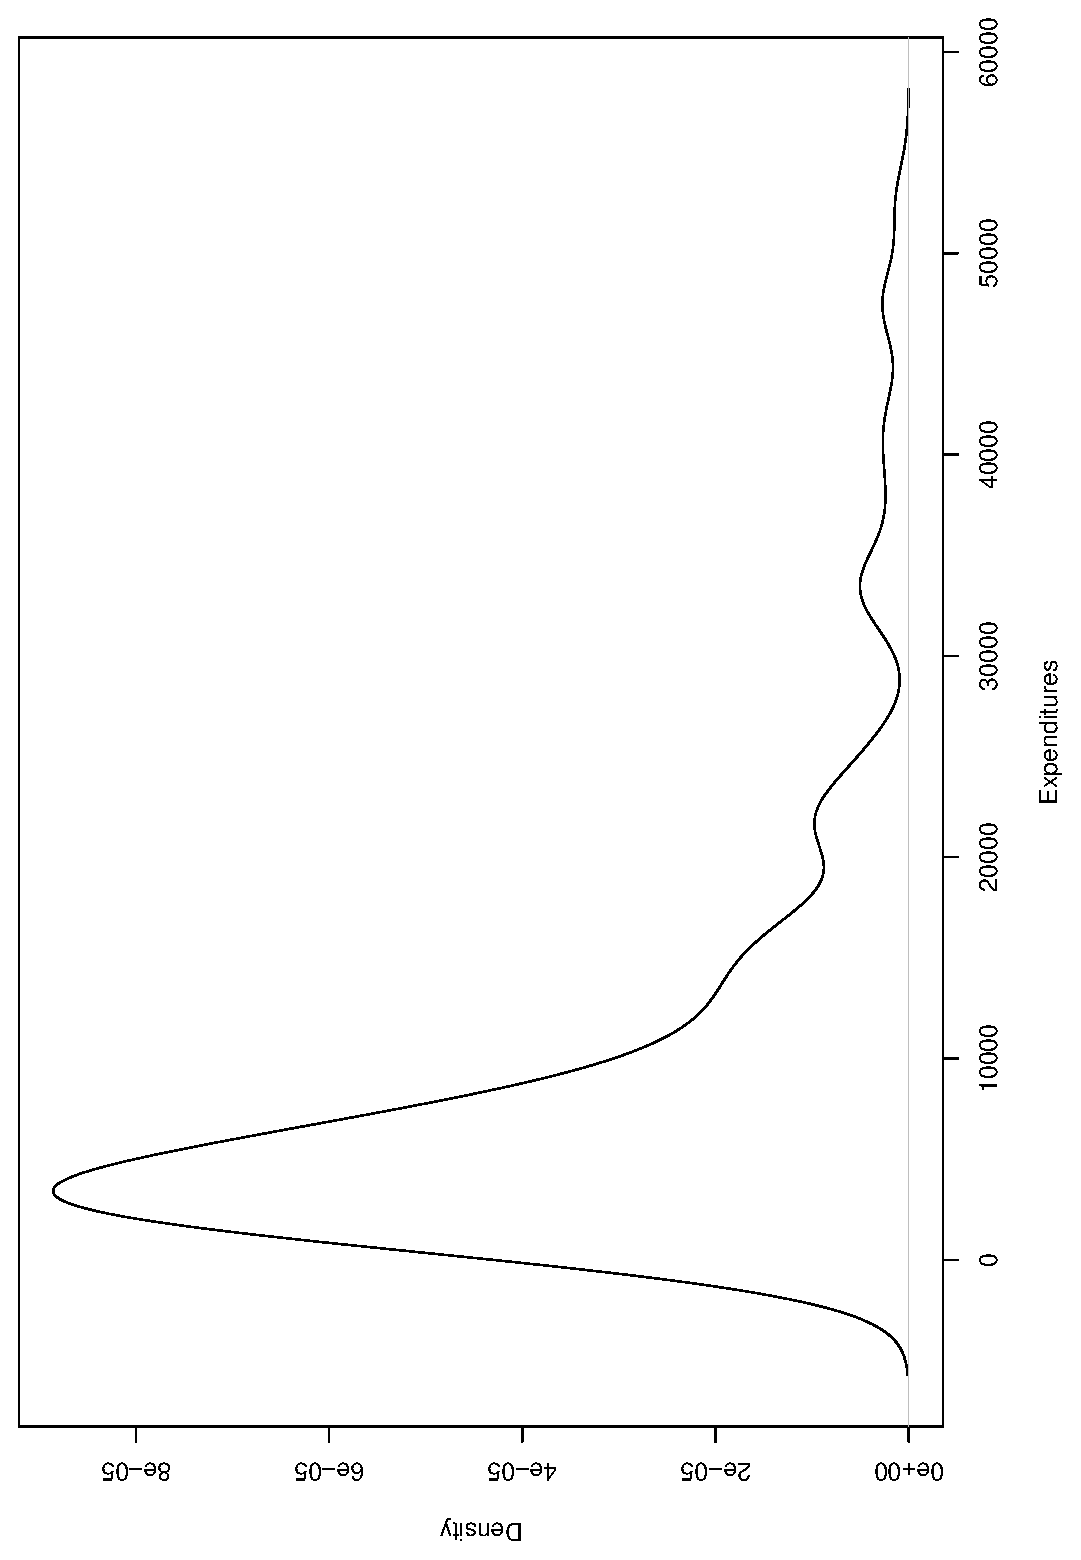
\includegraphics[width=1\textwidth,angle=270,scale=0.6]{Chapter13GLM/Fig13kernelExpendIP.eps}
    \caption{\label{F13:MEPSkernelExpendIP} \small Smooth Empirical
    Histogram of Positive Inpatient Expenditures. The largest
    expenditure is omitted.}
  \end{center}
\end{figure}

A gamma regression model using a logarithmic link was fit to
inpatient expenditures using all explanatory variables. The result
of this model fit appear in Table \ref{T13:MEPSLongTailModels}.
Here, we see that many of the potentially important determinants of
medical expenditures are not statistically significant. This is
common in expenditure analysis, where variables help predict the
frequency although are not as useful in explaining severity.

Because of collinearity, we have seen in linear models that having
too many variables in a fitted model can lead to statistical
insignificance of important variables and even cause signs to be
reversed. For a simpler model, we removed the Asian, Native American
and the uninsured variables because they account for a small subset
of our sample. We also used only the POOR variable for self-reported
health status and only POORNEG for income, essentially reducing
these categorical variables to binary variables. Table
\ref{T13:MEPSLongTailModels}, under the heading ``Reduced Model,''
reports the result of this model fit. This model has almost the same
goodness of fit statistic, $AIC$, suggesting that it is a reasonable
alternative. Under the reduced model fit, the variables COUNTIP
(inpatient count), AGE, COLLEGE and POORNEG, are statistically
significant variables. For these significant variables, the signs
are intuitively appealing. For example, the positive coefficient
associated with COUNTIP means that as the number of inpatient visits
increases, the total expenditures increases, as anticipated.

For another alternative model specification, Table
\ref{T13:MEPSLongTailModels} also shows a fit of an inverse gaussian
model with a logarithmic link. From the $AIC$ statistic, we see that
this model does not fit nearly as well as the gamma regression
model. All variables are statistically insignificant, making it
difficult to interpret this model.




\begin{table}[h]\begin{center}
\caption{\label{T13:MEPSLongTailModels} Comparison of Gamma and
Inverse Gaussian Regression Models} \scalefont{0.9}
\begin{tabular}{l|rr|rr|rr}
\hline & \multicolumn{4}{|c|}{Gamma} & \multicolumn{2}{|c}{Inverse Gaussian} \\
\hline & \multicolumn{2}{|c|}{Full Model} &
\multicolumn{2}{|c|}{Reduced Model} & \multicolumn{2}{|c}{Reduced
Model} \\ \cline{2-7}
& Parameter &  & Parameter &  & Parameter &  \\
Effect & Estimate & \textit{t}-value & Estimate & \textit{t}-value &
Estimate & \textit{t}-value \\ \hline
 Intercept &      6.891 &     13.080 &      7.859 &     17.951 &      6.544 &      3.024 \\
   COUNTIP &      0.681 &      6.155 &      0.672 &      5.965 &      1.263 &      0.989 \\
       AGE &      0.021 &      3.024 &      0.015 &      2.439 &      0.018 &      0.727 \\
    GENDER &     -0.228 &     -1.263 &     -0.118 &     -0.648 &      0.363 &      0.482 \\
     ASIAN &     -0.506 &     -1.029 &            &            &            &            \\
     BLACK &     -0.331 &     -1.656 &     -0.258 &     -1.287 &     -0.321 &     -0.577 \\
    NATIVE &     -1.220 &     -2.217 &            &            &            &            \\
 NORTHEAST &     -0.372 &     -1.548 &     -0.214 &     -0.890 &      0.109 &      0.165 \\
   MIDWEST &      0.255 &      1.062 &      0.448 &      1.888 &      0.399 &      0.654 \\
     SOUTH &      0.010 &      0.047 &      0.108 &      0.516 &      0.164 &      0.319
     \\\hline
   COLLEGE &     -0.413 &     -1.723 &     -0.469 &     -2.108 &     -0.367 &     -0.606 \\
HIGHSCHOOL &     -0.155 &     -0.827 &     -0.210 &     -1.138 &
-0.039 &     -0.078 \\\hline
      POOR &     -0.003 &     -0.010 &      0.167 &      0.706 &      0.167 &      0.258 \\
      FAIR &     -0.194 &     -0.641 &            &            &            &            \\
      GOOD &      0.041 &      0.183 &            &            &            &            \\
     VGOOD &      0.000 &      0.000 &            &            &            &            \\
   MNHPOOR &     -0.396 &     -1.634 &     -0.314 &     -1.337 &     -0.378 &     -0.642 \\
  ANYLIMIT &      0.010 &      0.053 &      0.052 &      0.266 &      0.218 &      0.287 \\\hline
   MINCOME &      0.114 &      0.522 &            &            &            &            \\
   LINCOME &      0.536 &      2.148 &            &            &            &            \\
     NPOOR &      0.453 &      1.243 &            &            &            &            \\
   POORNEG &     -0.078 &     -0.308 &     -0.406 &     -2.129 &     -0.356 &     -0.595 \\
    INSURE &      0.794 &      3.068 &            &            &            &            \\\hline
     Scale &      1.409 &      9.779 &      1.280 &      9.854 &      0.026 &     17.720 \\ \hline
Log-Likelihood & \multicolumn{2}{|c|}{-1,558.67 } &
\multicolumn{2}{|c|}{ -1,567.93  } & \multicolumn{2}{|c}{-1,669.02 } \\
\textit{AIC} & \multicolumn{2}{|c|}{  3,163.34} &
\multicolumn{2}{|c|}{  3,163.86} & \multicolumn{2}{|c}{ 3,366.04} \\
\hline
\end{tabular}\end{center}\scalefont{1.1111}\end{table}


\bigskip


\newpage

\section{Residuals}

One way of selecting an appropriate model is to fit a tentative
specification and analyze ways of improving it. This diagnostic
method relies on residuals. In the linear model, we defined
residuals as the response minus the corresponding fitted values. In
a GLM context, we refer to these as ``raw residuals,'' denoted as
$y_i - \widehat{\mu}_i$. As we have seen, residuals are useful for:
\begin{itemize}
\item discovering new covariates or the effects of nonlinear
patterns in existing covariates,
\item identifying poorly fitting observations,
\item quantifying the effects of individual observations on model
parameters and
\item revealing other model patterns, such as heteroscedasticity or
time trends.
\end{itemize}
As this section emphasizes, residuals are also the building blocks
for many goodness of fit statistics.

As we saw in Section 11.1 on binary dependent variables, analysis of
raw residuals can be meaningless in some nonlinear contexts. Cox and
Snell (1968, 1971) introduced a general notion of residuals that is
more useful in nonlinear models than the simple raw residuals. For
our applications, we assume that $y_i$ has a distribution function
F($\cdot$) that is indexed by explanatory variables $\mathbf{x}_i$
and a vector of parameters $\boldsymbol \theta$ denoted as
F($\mathbf{x}_i,\boldsymbol \theta$). Here, the distribution
function is common to all observations but the distribution varies
through the explanatory variables. The vector of parameters
$\boldsymbol \theta$ includes the regression parameters $\boldsymbol
\beta$ as well as scale parameters. With knowledge of F($\cdot$), we
now assume that a new function R($\cdot$) can be computed such that
$\varepsilon_i = \mathrm{R}(y_i; \mathbf{x}_i,\boldsymbol \theta)$,
where $\varepsilon_i$ are identically and independently distributed.
Here, the function R($\cdot$) depends on explanatory variables
$\mathbf{x}_i$ and parameters $\boldsymbol \theta$. The Cox-Snell
residuals are then $e_i = \mathrm{R}(y_i;
\mathbf{x}_i,\widehat{\boldsymbol \theta})$. If the model is
well-specified and the parameter estimates $\widehat{\boldsymbol
\theta}$ are close to the model parameters $\boldsymbol \theta$,
then the residuals $e_i$ should be close to i.i.d.

\index{residual!Cox-Snell}\index{residual!Pearson}\index{residual!Anscombe}

To illustrate, in the linear model we use the residual function
$\mathrm{R}(y_i; \mathbf{x}_i,\boldsymbol \theta) = y_i -
\mathbf{x}_i^{\prime} \boldsymbol \beta =y_i - \mu_i =
\varepsilon_i,$ resulting in (ordinary) raw residuals. Another
choice is to rescale by the standard deviation
\begin{equation*}
\mathrm{R}(y_i; \mathbf{x}_i,\boldsymbol \theta) = \frac{y_i -
\mu_i}{\sqrt{\mathrm{Var~} y_i}} , \end{equation*} that yields
\emph{Pearson residuals}.

Another type of residual is based on a first transforming the
response with a known function h($\cdot$),
\begin{equation*}
\mathrm{R}(y_i; \mathbf{x}_i,\boldsymbol \theta) =
\frac{\mathrm{h}(y_i) - \mathrm{E~}
\mathrm{h}(y_i)}{\sqrt{\mathrm{Var~}\mathrm{h}(y_i)}} .
\end{equation*}
Choosing the function so that h($y_i$) is approximately normally
distributed yields \emph{Anscombe residuals}. Another popular choice
is to choose the transform so that the variance is stabilized. Table
\ref{T13:ResidualTransforms} gives transforms for the binomial,
Poisson and gamma distributions.

\index{transformations!approximate
normality}\index{transformations!variance-stabilizing}

\begin{table}[h]
\caption{\label{T13:ResidualTransforms} Approximate Normality and
Variance-Stabilizing Transforms}
\begin{tabular}{lcc}
\hline
Distribution & Approximate Normality & Variance-Stabilizing \\
 & Transform & Transform \\
\hline Binomial($m,p$) &
$\frac{\mathrm{h}_B(y/m)-[\mathrm{h}_B(p)+(p(1-p))^{-1/3}(2p-1)/(6m)]}{(p(1-p)^{1/6}/\sqrt{m}}$
&
$\frac{\sin^{-1}(\sqrt{y/m})-\sin^{-1}(\sqrt{p})}{a/(2\sqrt{m})}$ \smallskip\\
Poisson($\lambda$) & $1.5 \lambda^{-1/6} \left[
y^{2/3}-(\lambda^{2/3}-\lambda^{-1/3}/9) \right] $ &
$ 2(\sqrt{y}-\sqrt{\lambda})$\\
Gamma($\alpha, \gamma$) & $ 3 \alpha^{1/6} \left[
(y/\gamma)^{1/3}-(\alpha^{1/3}-\alpha^{-2/3}/9) \right]$
& Not considered\\
\hline \multicolumn{3}{l}{Note: $\mathrm{h}_B(u) = \int_0^u s^{-1/3}
(1-s)^{-1/3}ds$
is the incomplete beta function evaluated at (2/3, 2/3), }\\
\multicolumn{3}{l}{~~~up to a scalar constant. \emph{Source: Pierce and Schafer (1986)}. } \\
 \hline
\end{tabular}
\end{table}

\index{residual!deviance}

Another widely used choice in GLM studies are \emph{deviance
residuals}, defined as
\begin{equation*}\mathrm{sign} \left(y_i -
\widehat{\mu}_i \right)
 \sqrt{2  \left( \ln \mathrm{f}(y_i;\theta_{i,SAT}) - \ln
 \mathrm{f}(y_i;\widehat{\theta}_{i})
 \right)}.
 \end{equation*}
Section \ref{S13:Goodness} introduced the parameter estimates of the
saturated model, $\theta_{i,SAT}$. As discussed by Pierce and
Schafer (1986), deviance residuals are very close to Anscombe
residuals in many cases - we can check deviance residuals for
approximate normality. Further, deviance residuals can be defined
readily for any GLM model and are easy to compute.


%\subsection{Automatic Variable Selection Procedures}
%Leaps and Bounds Algorithm


\section{Tweedie Distribution}\label{S13:Tweedie}\index{regression model!Tweedie $GLM$}
\index{distributions!Tweedie}

We have seen that the natural exponential family includes continuous
distributions, such as the normal and gamma, as well as discrete
distributions, such as the binomial and Poisson. It also includes
distributions that are mixtures of discrete and continuous
components. In insurance claims modeling, the most widely used
mixture is the Tweedie (1984) distribution. It has a positive mass
at zero representing no claims and a continuous component for
positive values representing the amount of a claim.

The Tweedie distribution is defined as a Poisson sum of gamma random
variables, known as an \emph{aggregate loss} in actuarial science.
Specifically, suppose that $N$ has a Poisson distribution with mean
$\lambda$, representing the number of claims. Let {$y_j$} be an
i.i.d. sequence, independent of $N$, with each $y_j$ having a gamma
distribution with parameters $\alpha$ and $\gamma$, representing the
amount of a claim. Then, $S_N = y_1 + \ldots + y_N$ is Poisson sum
of gammas. Section 16.5 will discuss aggregate loss models in
further detail. This section focuses on the important special case
of the Tweedie distribution.

To understand the mixture aspect of the Tweedie distribution, first
note that it is straightforward to compute the probability of zero
claims as
\begin{equation*}
\Pr ( S_N=0) = \Pr (N=0) = e^{-\lambda}.
\end{equation*}
The distribution function can be computed using conditional
expectations,
\begin{equation*}
\Pr ( S_N \leq y) = e^{-\lambda}+\sum_{n=1}^{\infty} \Pr(N=n)
\Pr(S_n \leq y), ~~~~~y \geq 0.
\end{equation*}
Because the sum of i.i.d. gammas is a gamma, $S_n$ (not $S_N$) has a
gamma distribution with parameters $n\alpha$ and $\gamma$. Thus, for
$y>0$, the density of the Tweedie distribution is
\begin{equation}\label{E13:TweedieDensity1}
\mathrm{f}_{S}(y) = \sum_{n=1}^{\infty} e^{-\lambda} \frac{\lambda
^n}{n!} \frac{\gamma^{n \alpha}}{\Gamma(n \alpha)} y^{n \alpha -1}
e^{-y \gamma}.
\end{equation}

At first glance, this density does not appear to be a member of the
linear exponential family given in equation
(\ref{E13:LinearExpFam}). To see the relationship, we first
calculate the moments using iterated expectations as
\begin{equation}\label{E13:MomentsTweedie}
\mathrm{E~}S_N = \lambda
\frac{\alpha}{\gamma}~~~~~~\mathrm{and}~~~~~ \mathrm{Var~}S_N =
\frac{\lambda \alpha}{\gamma^2} (1+\alpha).
\end{equation}
Now, define three parameters $\mu, \phi,  p$ through the relations
\begin{equation*}
\lambda = \frac{\mu^{2-p}}{\phi (2-p)},~~~~~~\alpha =
\frac{2-p}{p-1}~~~~~~\mathrm{and}~~~~~ \frac{1}{\gamma} =
\phi(p-1)\mu^{p-1}.
\end{equation*}
Inserting these new parameters in equation
(\ref{E13:TweedieDensity1}) yields
\begin{equation}\label{E13:TweedieDensity2}
\mathrm{f}_{S}(y) = \exp \left[ \frac{-1}{\phi} \left(
\frac{\mu^{2-p}}{2-p} + \frac{y}{(p-1)\mu^{p-1}} \right) +S(y,\phi)
\right].
\end{equation}
We leave the calculation of $S(y,\phi)$ as an exercise.

Thus, the Tweedie distribution is a member of the linear exponential
family. Easy calculations show that
\begin{equation}\label{E13:MomentsTweedie}
\mathrm{E~}S_N = \mu~~~~~~\mathrm{and}~~~~~ \mathrm{Var~}S_N = \phi
\mu^p,
\end{equation}
where $1<p<2.$ Examining our variance function Table
\ref{T13:VarianceFunctions}, the Tweedie distribution can also be
viewed as a choice that is intermediate between the Poisson and the
gamma distributions.


\section{Further Reading and References}

A more extensive treatment of GLM may be found in the classic work
by McCullagh and Nelder (1989) or the gentler introduction by Dobson
(2002). de Jong and Heller (2008) provide a recent book-long
introduction to GLMs with a special insurance emphasis.

GLMs have enjoyed substantial attention from property and casualty
(general) insurance practicing actuaries recently, see Anderson et
al. (2004) and Clark and Thayer (2004) for introductions.

Mildenhall (1999) provides a systematic analysis of the connection
between GLM models and algorithms for assessing different rating
plans. Fu and Wu (2008) provide an updated version, introducing a
broader class of iterative algorithms that tie nicely to GLM models.

For further information on the Tweedie distribution, see
J{\o}rgensen and de Souza (1994) and Smyth and J{\o}rgensen (2002).

\bigskip

\textbf{Chapter References}

\begin{multicols}{2}

\scalefont{0.9}

Anderson, Duncan, Sholom Feldblum, Claudine Modlin, Doris
Schirmacher, Ernesto Schirmacher and Neeza Thandi (2004). A
practitioner's guide to generalized linear models. \textit{Casualty
Actuarial Society 2004 Discussion Papers} 1-116, Casualty Actuarial
Society.

Baxter, L. A., S. M. Coutts and G. A. F. Ross (1980). Applications
of linear models in motor insurance. \textit{Proceedings of the 21st
International Congress of Actuaries.} Zurich. pp. 11-29.

Clark, David R. and Charles A. Thayer (2004). A primer on the
exponential family of distributions. \textit{Casualty Actuarial
Society 2004 Discussion Papers} 117-148, Casualty Actuarial Society.

Cox, David R. and E. J. Snell (1968). A general definition of
residuals. \emph{Journal of the Royal Statistical Society}, Series
B, 30, 248-275.

Cox, David R. and E. J. Snell (1971). On test statistics computed
from residuals. \emph{Biometrika} 71, 589-594.

Dobson, Annette J. (2002). \textit{An Introduction to Generalized
Linear Models, Second Edition.} Chapman \& Hall, London.

Fu, Luyang and Cheng-sheng Peter Wu (2008). General iteration
algorithm for classification ratemaking. \textit{Variance} 1(2),
193-213, Casualty Actuarial Society.

de Jong, Piet and Gillian Z. Heller (2008). \textit{Generalized
Linear Models for Insurance Data}. Cambridge University Press,
Cambridge, UK.

J{\o}rgensen, Bent and Marta C. Paes de Souza (1994). Fitting
Tweedie's compound Poisson model to insurance claims data.
\emph{Scandinavian Actuarial Journal} 1994;1, 69-93.

McCullagh, P. and J.A. Nelder (1989). \textit{Generalized Linear
Models, Second Edition.} Chapman \& Hall, London.

Mildenhall, Stephen J. (1999). A systematic relationship between
minimum bias and generalized linear models. \textit{Casualty
Actuarial Society Proceedings} 86, Casualty Actuarial Society.

Pierce, Donald A. and Daniel W. Schafer (1986). Residuals in
generalized linear models. \emph{Journal of the American Statistical
Association} 81, 977-986.

Smyth, Gordon K. and Bent J{\o}rgensen (2002). Fitting Tweedie's
compound Poisson model to insurance claims data: Dispersion
modelling. \emph{Astin Bulletin} 32(1), 143-157.

Tweedie, M. C. K. (1984). An index which distinguishes between some
important exponential families. In \emph{Statistics: Applications
and New Directions}. \emph{Proceedings of the Indian Statistical
Golden Jubilee International Conference} (Editors J. K. Ghosh and J.
Roy), pp. 579-604. Indian Statistical Institute, Calcutta.

\scalefont{1.1111}

\end{multicols}


\section{Exercises}

\begin{exercises}

\scalefont{0.90}

\item Verify the entries in Table \ref{T13:SelDistns} for the gamma
distribution. Specifically:

a. Show that the gamma is a member of the linear exponential family
of distributions.

b. Describe the components of the linear exponential family ($
\theta, \phi, b(\theta), S(y,\phi)$) in terms of the parameters of
the gamma distribution.

c. Show that the mean and variance of the gamma and linear
exponential family distributions agree.

\empexjed{AutoCollision}

\item \textbf{Ratemaking Classification}. This exercise considers the
data described in the Section \ref{S13:LinkFunction} ratemaking
classification example using data in Table
\ref{T13:PrivateCollision}.

a. Fit a gamma regression model using a log-link function with claim
counts as weights ($w_i$). Use the categorical explanatory variables
age group and vehicle use to estimate expected average severity.

b. Based on your estimated parameters in part (a), verify the
estimated expected severities in Table
\ref{T13:PrivateCollisionRates}.

\item Verify that the Tweedie distribution is a member of the linear exponential family
of distributions by checking equation (\ref{E13:TweedieDensity1}).
In particular, provide an expression for $S(y,\phi)$ (note that
$S(y,\phi)$ also depends on $p$ but not on $\mu$). You may wish to
see Clark and Thayer (2004) to check your work. Further, verify the
moments in equation (\ref{E13:MomentsTweedie}).



 \scalefont{1.1111}

\end{exercises}


\section{Technical Supplements - Exponential Family}

\subsection{Linear Exponential Family of Distributions}
The distribution of the random variable $y$ may be discrete,
continuous or a mixture. Thus, f(.) in equation
(\ref{E13:LinearExpFam}) may be interpreted to be a density or mass
function, depending on the application. Table \ref{T13:SelDistns}
provides several examples, including the normal, binomial and
Poisson distributions.


\clearpage

\begin{landscape}

\scalefont{0.9}
\begin{table}[h]
\caption{\label{T13:SelDistns} Selected Distributions of the
One-Parameter Exponential Family}
\begin{center}
\begin{tabular}{l|ccccc}
\hline
             &             & Density or & & & \\
Distribution & Parameters & Mass Function & Components & $\mathrm{E}~y$ & $\mathrm{Var}~y$ \\
\hline General & $\theta,~ \phi$ &
$\exp \left( \frac{y\theta -b(\theta )}{\phi }%
+S\left( y,\phi \right) \right) $
 & $\theta,~ \phi, b(\theta), S(y, \phi)$ & $b^{\prime}(\theta)$ & $b^{\prime \prime}(\theta) \phi $\\
 Normal & $\mu, \sigma^2 $&
$ \frac{1}{\sigma \sqrt{2\pi }}\exp \left( -%
\frac{(y-\mu )^{2}}{2\sigma ^{2}}\right)$ & $\mu, \sigma^2,
\frac{\theta^2}{2}, - \left(\frac{y^2}{2\phi} + \frac{\ln(2 \pi
\phi)}{2} \right) $& $\theta=\mu$ & $\phi= \sigma^2 $ \\
Binomal & $\pi$ & ${n \choose y} \pi ^y (1-\pi)^{n-y}$ & $\ln
\left(\frac{\pi}{1-\pi} \right), 1, n \ln(1+e^{\theta} ), $ & $n
\frac {e^{\theta}}{1+e^{\theta}}  $& $n \frac
{e^{\theta}}{(1+e^{\theta})^2} $ \\
&  &  & $ \ln {n \choose y} $ & $ = n \pi $& $ = n \pi (1-\pi)$ \\
Poisson & $\lambda$ & $ \frac{\lambda^y}{y!} \exp(-\lambda) $ & $
\ln \lambda, 1, e^{\theta}, - \ln (y!) $ & $e^{\theta} = \lambda $ &
$e^{\theta} = \lambda $ \\
Negative Binomial$^{\ast}$ & $r,p$ & $ \frac{\Gamma(y+r)}{y!
\Gamma(r)} p^r ( 1-p)^y$ & $\ln(1-p), 1, -r \ln(1-e^{\theta}),$ &
$\frac{r(1-p)}{p}$
& $\frac{r(1-p)}{p^2} $ \\
 & & & ~~~$\ln \left[ \frac{\Gamma(y+r)}{y!
\Gamma(r)} \right]$ & \multicolumn{1}{r}{= $\mu $} &
\multicolumn{1}{r}{= $\mu+\mu^2/r$}
\\
Gamma & $\alpha, \gamma $ & $\frac{\gamma ^ \alpha}{\Gamma (\alpha)}
y^{\alpha -1 }\exp(-y \gamma) $ & $- \frac{\gamma}{\alpha},
\frac{1}{\alpha}, - \ln ( - \theta), -\phi^{-1} \ln \phi$ & $ -
\frac{1}{\theta} = \frac{\alpha}{\gamma} $ &$ \frac{\phi}{\theta ^2}
=
\frac{\alpha}{\gamma ^2} $ \\
& & & $ - \ln \left( \Gamma(\phi ^{-1}) \right) +
(\phi^{-1} - 1) \ln y $& & \\
Inverse Gaussian & $\mu, \lambda$ & $\sqrt{\frac{\lambda}{2 \pi y^3}
} \exp \left(- \frac{\lambda (y-\mu)^2}{2 \mu^2 y} \right) $ & $
-1/( 2\mu^2), 1/\lambda, -\sqrt{-2 \theta}, $ & $ \left(-2 \theta
\right)^{-1/2} $ & $
\phi (-2 \theta)^{-3/2}  $\\
 &  & & $ \theta/(\phi y) - 0.5 \ln
(\phi 2 \pi y^3 )$ & \multicolumn{1}{r}{= $\mu$} &
\multicolumn{1}{r}{= $\frac{\mu^3}{\lambda}$} \\
Tweedie & \multicolumn{3}{l}{See Section \ref{S13:Tweedie}}\\
 \hline
 \multicolumn{3}{l}{$^{\ast}$ This assumes that the parameter $r$ is fixed but need not be an integer.}\\
 \hline

\end{tabular}\end{center}\end{table}
\scalefont{1.1111}

\end{landscape}

\subsection{Moments}\label{S13:Moments}

To assess the moments of exponential families, it is convenient to
work with the moment generating function. For simplicity, we assume
that the random variable $y$ is continuous. Define the moment
generating function

\begin{eqnarray*}
M(s) &=& \mathrm{E}~ e^{sy} = \int \exp \left( sy+ \frac{y \theta -
b(\theta)}{\phi} + S(y, \phi) \right) dy \\
&=& \exp \left(\frac{b(\theta + s \phi) - b(\theta)}{\phi} \right)
\int \exp \left( \frac{y(\theta + s\phi) - b(\theta+s\phi)}{\phi} +
S(y, \phi) \right) dy \\
&=& \exp \left(\frac{b(\theta + s \phi) - b(\theta)}{\phi} \right),
\end{eqnarray*}
because $\int \exp \left( \frac{1}{\phi} \left[ y(\theta + s\phi) -
b(\theta+s\phi) \right] + S(y, \phi) \right) dy=1$. With this
expression, we can generate the moments. Thus, for the mean, we have
\begin{eqnarray*}
\mathrm{E}~ y &=& M^{\prime}(0) =  \left . \frac{\partial}{\partial
s} \exp \left(\frac{b(\theta + s \phi) - b(\theta)}{\phi} \right)
\right | _{s=0} \\
&=& \left[ b^{\prime}(\theta + s \phi ) \exp \left( \frac{b(\theta +
s \phi) - b(\theta)}{\phi} \right) \right] _{s=0} =
b^{\prime}(\theta).
\end{eqnarray*}

Similarly, for the second moment, we have
\begin{eqnarray*}
M^{\prime \prime}(s) &=&  \frac{\partial}{\partial s} \left[
b^{\prime}(\theta + s \phi) \exp \left(\frac{b(\theta + s \phi) -
b(\theta)}{\phi} \right) \right]  \\
&=& \phi b^{\prime \prime}(\theta + s \phi) \exp
\left(\frac{b(\theta + s \phi) - b(\theta)}{\phi} \right) +
(b^{\prime}(\theta + s \phi))^2 \left(\frac{b(\theta + s \phi) -
b(\theta)}{\phi} \right).
\end{eqnarray*}
This yields $\mathrm{E}y^2 = M^{\prime \prime}(0) = \phi b^{\prime
\prime}(\theta) + (b^{\prime}(\theta))^2 $ and $ \mathrm{Var}~y =
\phi b^{\prime \prime}(\theta)$.

\subsection{Maximum Likelihood Estimation for General
Links}\label{S13:MLEGeneralLinks}\index{likelihood inference!maximum
likelihood estimator}

For general links, we no longer assume the relationship $\theta_i=\mathbf{%
x}_i^{\mathbf{\prime }}\boldsymbol \beta$ but assume that
$\boldsymbol \beta$ is related to $\theta_i$ through the relations
$\mu _i=b^{\prime }(\theta_i)$ and $\mathbf{x}_i^{\mathbf{\prime
}}\boldsymbol \beta = g\left( \mu _i\right) $. We continue to assume
that the scale parameter varies by observation so that $\phi_i =
\phi/w_i$, where $w_i$ is a known weight function. Using equation
(\ref{E13:LogLike}), we have that the $j$th element of the score
function is
\[
\frac{\partial }{\partial \beta _{j}}\ln \mathrm{f}\left(
\mathbf{y}\right)
=\sum_{i=1}^n  \frac{\partial \theta_i}{\partial \beta _{j}}%
\frac{y_i-\mu _i}{\phi _i} ,
\]%
because $b^{\prime }(\theta_i)=\mu _i$. Now, use the chain rule and
the
relation $\mathrm{Var~}y_i=\phi _ib^{\prime \prime }(\theta_i)$ to get%
\[
\frac{\partial \mu _i}{\partial \beta _{j}}=\frac{\partial b^{\prime
}(\theta_i)}{\partial \beta _{j}}=b^{\prime \prime }(\theta_i)\frac{%
\partial \theta_i}{\partial \beta _{j}}=\frac{\mathrm{Var~}y_i}{\phi
_i}\frac{\partial \theta_i}{\partial \beta _{j}}.
\]%
Thus, we have
\[
\frac{\partial \theta_i}{\partial \beta _{j}}\frac{1}{\phi _i}=\frac{%
\partial \mu _i}{\partial \beta _{j}}\frac{1}{\mathrm{Var~}y_i}.
\]
This yields
\begin{equation*}
\frac{\partial }{\partial \beta _{j}}\ln \mathrm{f}\left(
\mathbf{y}\right) =\sum_{i=1}^n  \frac{\partial \mu _i}{\partial
\beta _{j}}\left( \mathrm{Var~}y_i\right) ^{-1}\left( y_i-\mu
_i\right)  ,
\end{equation*}
that we summarize as\setcounter{equation}{12}
\begin{equation}\label{E13:GeneralScore}
\frac{\partial  L(\boldsymbol \beta) }{\partial \boldsymbol \beta }
=  \frac{\partial }{\partial \boldsymbol \beta }\ln \mathrm{f}\left(
\mathbf{y}\right) =\sum_{i=1}^n  \frac{\partial \mu _i}{\partial
\boldsymbol \beta}\left( \mathrm{Var~}y_i\right) ^{-1}\left( y_i-\mu
_i\right) ,
\end{equation}
which is known as the \emph{generalized estimating equations}
form.\index{likelihood inference!generalized estimating equations}

Solving for roots of the score equation $L(\boldsymbol \beta) =
\mathbf{0}$ yield maximum likelihood estimates, $\mathbf{b}_{MLE}$.
In general, this requires iterative numerical methods. An exception
is the following special case.

\linejed

\textbf{Special Case. No Covariates.} Suppose that $k=1$ and that
$x_i =1$. Thus, $\beta = \eta = g(\mu),$ and $\mu$ does not depend
on $i$. Then, from the relation $\mathrm{Var~}y_i = \phi b^{\prime
\prime}(\theta)/w_i$  and equation (\ref{E13:GeneralScore}), the
score function is
\begin{equation*}
\frac{\partial  L( \beta) }{\partial \beta } = \frac{\partial
\mu}{\partial \beta} ~ \frac{1}{\phi b^{\prime \prime}(\theta)}
\sum_{i=1}^n w_i \left( y_i-\mu \right) .
\end{equation*}
Setting this equal zero yields $\overline{y}_w = \sum_i w_i y_i /
\sum_i w_i = \widehat{\mu}_{MLE} = g^{-1}(b_{MLE})$, or
$b_{MLE}=g(\overline{y}_w),$ where $\overline{y}_w $ is a weighted
average of $y$'s.

\linejed\index{likelihood inference!information matrix}

For the information matrix, use the independence among subjects and
equation (\ref{E13:GeneralScore}) to get
\begin{eqnarray}\label{E13:GLMHessian}
\mathbf{I}(\boldsymbol \beta)
 &=& \mathrm{E~} \left( \frac{\partial
L(\boldsymbol \beta) }{\partial \boldsymbol \beta } \frac{\partial
L(\boldsymbol \beta) }{\partial \boldsymbol \beta ^{\prime}} \right) \nonumber \\
&=& \sum_{i=1}^n \frac{\partial \mu _i}{\partial \boldsymbol
\beta}~\mathrm{E} \left( \left( \mathrm{Var~}y_i\right) ^{-1}\left(
y_i-\mu _i\right)^2 \left( \mathrm{Var~}y_i\right) ^{-1}\right)
\frac{\partial \mu _i}{\partial
\boldsymbol \beta ^{\prime}} \nonumber \\
&=& \sum_{i=1}^n \frac{\partial \mu _i}{\partial \boldsymbol \beta}
\left( \mathrm{Var~}y_i\right) ^{-1} \frac{\partial \mu _i}{\partial
\boldsymbol \beta ^{\prime}} .
\end{eqnarray}

Taking the square root of the diagonal elements of the inverse of $\mathbf{I}(\boldsymbol \beta)$,
after inserting parameter estimates in the mean and variance functions, yields
\emph{model-based standard errors}. For data where the correct specification of the variance component
is in doubt, one replaces Var $y_i$ by an unbiased estimate $(y_i - \mu_i)^2$. The resulting estimator
\begin{equation*}
se(b_j) = \sqrt{ jth~diagonal~element~of~
[\sum_{i=1}^n \frac{\partial \mu _i}{\partial \boldsymbol \beta}
 (y_i - \mu_i)^{-2} \frac{\partial \mu _i}{\partial
\boldsymbol \beta ^{\prime}}
]|_{\boldsymbol \beta = \mathbf{b}_{MLE}}^{-1}}
\end{equation*}

is known as the \emph{empirical, or robust, standard
error}.\index{likelihood inference!robust standard
error}\index{likelihood inference!model-based standard errors}

\subsection{Iterated Reweighted Least Squares}\label{S13:IterRWLS}\index{least
squares!iterated reweighted}\index{likelihood
inference!Newton-Raphson algorithm}\index{matrix algebra!Hessian}

To see how general iterative methods work, we use the canonical link
so that $\eta_i = \theta_i$. Then, the score function is given in
equation (\ref{E13:GLMScore}) and the Hessian is in equation
(\ref{E13:StdErrors}). Using the Newton-Raphson equation (11.15) in
Section 11.9 yields
\begin{equation}\label{E13:NewtonRaphsonCanLink}
\boldsymbol \beta_{NEW} = \boldsymbol \beta_{OLD} -  \left(
\sum_{i=1}^n w_i b^{\prime \prime}(\mathbf{x}_i^{\prime} \boldsymbol
\beta _{OLD}) \mathbf{x}_i \mathbf{x}_i^{\prime} \right)^{-1} \left(
\sum_{i=1}^n w_i (y_i - b^{\prime}(\mathbf{x}_i^{\prime} \boldsymbol
\beta_{OLD})) \mathbf{x}_i \right) .
  \end{equation}
Note that because the matrix of second derivatives is
non-stochastic, the Newton-Raphson is equivalent to the Fisher
scoring algorithm. As described in Section \ref{S13:MLECanonLinks},
the estimation of $\boldsymbol \beta$ does not require knowledge of
$\phi$.


Continue using the canonical link and define an ``adjusted dependent
variable''
\begin{equation*}
y_i^{\ast}(\boldsymbol \beta) = \mathbf{x}_i^{\prime} \boldsymbol
\beta + \frac{y_i - b^{\prime}(\mathbf{x}_i^{\prime} \boldsymbol
\beta)}{b^{\prime \prime}(\mathbf{x}_i^{\prime} \boldsymbol \beta)}.
\end{equation*}
This has variance
\begin{equation*}
\mathrm{Var~}y_i^{\ast}(\boldsymbol \beta) =
\frac{\mathrm{Var~}y_i}{(b^{\prime \prime}(\mathbf{x}_i^{\prime}
\boldsymbol \beta))^2} = \frac{\phi_i b^{\prime
\prime}(\mathbf{x}_i^{\prime} \boldsymbol \beta)}{(b^{\prime
\prime}(\mathbf{x}_i^{\prime} \boldsymbol \beta))^2} = \frac{\phi/
w_i }{b^{\prime \prime}(\mathbf{x}_i^{\prime} \boldsymbol \beta)}.
\end{equation*}
Use the new weight as the reciprocal of the variance,
$w_i(\boldsymbol \beta)=w_i b^{\prime \prime}(\mathbf{x}_i^{\prime}
\boldsymbol \beta) / \phi.$ Then, with the expression
\begin{equation*}
w_i \left(y_i - b^{\prime}(\mathbf{x}_i^{\prime} \boldsymbol
\beta)\right) = w_i b^{\prime \prime}(\mathbf{x}_i^{\prime}
\boldsymbol \beta) (y_i^{\ast}(\boldsymbol \beta) -
\mathbf{x}_i^{\prime} \boldsymbol \beta) = \phi w_i(\boldsymbol
\beta) (y_i^{\ast}(\boldsymbol \beta) - \mathbf{x}_i^{\prime}
\boldsymbol \beta),
\end{equation*}
from the Newton-Raphson iteration in equation
(\ref{E13:NewtonRaphsonCanLink}), we have

\noindent $\boldsymbol \beta_{NEW}$
\begin{eqnarray*}
~ &=& \boldsymbol \beta_{OLD} -  \left( \sum_{i=1}^n w_i b^{\prime
\prime}(\mathbf{x}_i^{\prime} \boldsymbol \beta _{OLD}) \mathbf{x}_i
\mathbf{x}_i^{\prime} \right)^{-1} \left( \sum_{i=1}^n w_i (y_i -
b^{\prime}(\mathbf{x}_i^{\prime} \boldsymbol
\beta_{OLD})) \mathbf{x}_i \right) \\
&=& \boldsymbol \beta_{OLD} -  \left( \sum_{i=1}^n \phi
w_i(\boldsymbol \beta _{OLD}) \mathbf{x}_i \mathbf{x}_i^{\prime}
\right)^{-1} \left( \sum_{i=1}^n \phi w_i(\boldsymbol \beta _{OLD})
(y_i^{\ast}(\boldsymbol \beta_{OLD}) - \mathbf{x}_i^{\prime}
\boldsymbol \beta_{OLD})\mathbf{x}_i \right) \\
&=& \boldsymbol \beta_{OLD} -  \left( \sum_{i=1}^n w_i(\boldsymbol
\beta _{OLD}) \mathbf{x}_i \mathbf{x}_i^{\prime} \right)^{-1} \left(
\sum_{i=1}^n  w_i(\boldsymbol \beta _{OLD})\mathbf{x}_i
y_i^{\ast}(\boldsymbol \beta_{OLD}) - \sum_{i=1}^n w_i(\boldsymbol
\beta _{OLD})\mathbf{x}_i
\mathbf{x}_i^{\prime} \boldsymbol \beta_{OLD}) \right) \\
&=& \left( \sum_{i=1}^n  w_i(\boldsymbol \beta _{OLD}) \mathbf{x}_i
\mathbf{x}_i^{\prime} \right)^{-1} \left( \sum_{i=1}^n
w_i(\boldsymbol \beta _{OLD})\mathbf{x}_i y_i^{\ast}(\boldsymbol
\beta_{OLD})  \right).
  \end{eqnarray*}
Thus, this provides a method for iteration using weighted least
squares. Iterative reweighted least squares is also available for
general links using Fisher scoring, see McCullagh and Nelder (1989)
for further details.
